\chapter{Methods}
\label{chap:methods}
Here, we extensively explain the methods we used and propose to utilize SCADA log messages in wind turbine normal behavior machine learning models.
We start by introducing the dataset used to run the experiments.
Then, we define the concept of normal behavior modeling and the machine learning models and their architecture used in this work.
Finally, we introduce two different approaches to utilizing SCADA logs with ways of using them as input features in machine learning models, as s filter for the SCADA signals,
or to visualize relevant warnings.

\section{Dataset}
In this section, we will describe the dataset used in this work to train, test and validate the models. 
\par We used open-source data published on the \emph{EDP OpenData} web platform \cite{EDP} and that was made available for research purposes. 
The data was collected from the SCADA systems of five different Vestas wind turbines (Turbine 01, 06, 07, 09 and 11) in the same wind park between the years 2016 and 2017 
and is made up of the following four subsets: \emph{Signals, Logs, Failures and Metmast}. We will, however, only describe three sets since \emph{Metmast} was not used in this work.
A full description of the turbines' characteristics (e.g., rated power, cut-in speed, rotor diameter,\dots) and their power curve is documented in Appendix \ref{chap:appendix1}.

\subsection{Signals}
 The \emph{Signals} dataset contains 10-min aggregated data (Mean, STandard Deviation (STD), Minimum (Min), and Maximum (Max) values) collected from the wind turbines' power meters and
 sensors installed at the major components such as gearbox, generator and transformer (see Figure \ref{fig:WTG_Diagram} for a 
 demonstration of a turbine's hardware and the location of major components). These built-in sensors measure quantities such as temperatures, angles, wind and rotational speeds, 
 power production,\dots

 \begin{figure}[H]
  \begin{center}
    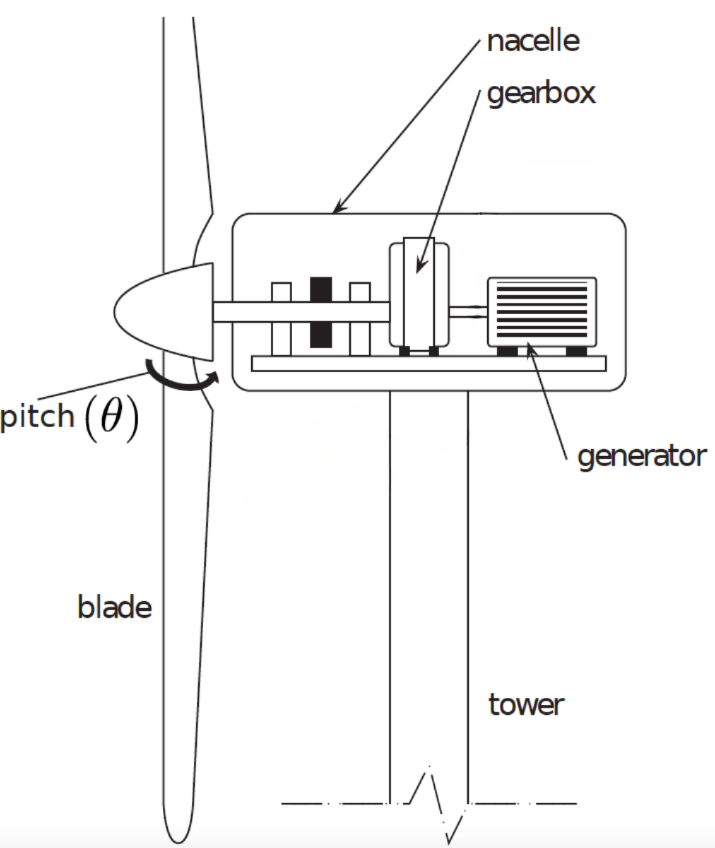
\includegraphics[scale=0.3]{Methods/Horizontal-axis-wind-turbine.png}
  \end{center}
  \caption{Diagram of a wind turbine side view with labeled main components. Figure adapted from \cite{WTG_Diagram}}
  \label{fig:WTG_Diagram}
\end{figure}

 This dataset was the most crucial for this work since it provides information that reflects the status of the turbine operation which is needed to perform 
 SCADA-based automated condition monitoring and predictive maintenance.\\
 Table \ref{tab:signals} shows some of the 81 signals included in this dataset and Figure \ref{fig:sample_signals} shows a sample of selected signals collected from Turbine 01 
 along with some statistics that describe the whole dataset.
 \begin{table}[H]
        \centering
    \begin{tabular}{ | m{12em} | m{8cm} | }
    \hline
         \multicolumn{1}{|c|}{\textbf{Type of signal}} & \multicolumn{1}{c|}{\textbf{Signals}} \\
         \hline
         Temperature (\degree C) & Generator, Generator bearings, Hydraulic group oil, Gearbox oil, Gearbox bearing on the high-speed shaft, 
         Nacelle, High Voltage (HV) transformer, Ambient temperature,\dots  \\
         \hline
         Production value & Active power in Wh, Reactive power in VArh, Power according to the grid in kW,\dots \\
         \hline
         Angle (\degree) & Blades pitch angle ($\theta$) \\
    \hline
    \end{tabular}
    \caption{Example signals found in the Signals dataset}
        \label{tab:signals}
  \end{table}

  \begin{figure}[H]
    \begin{center}
      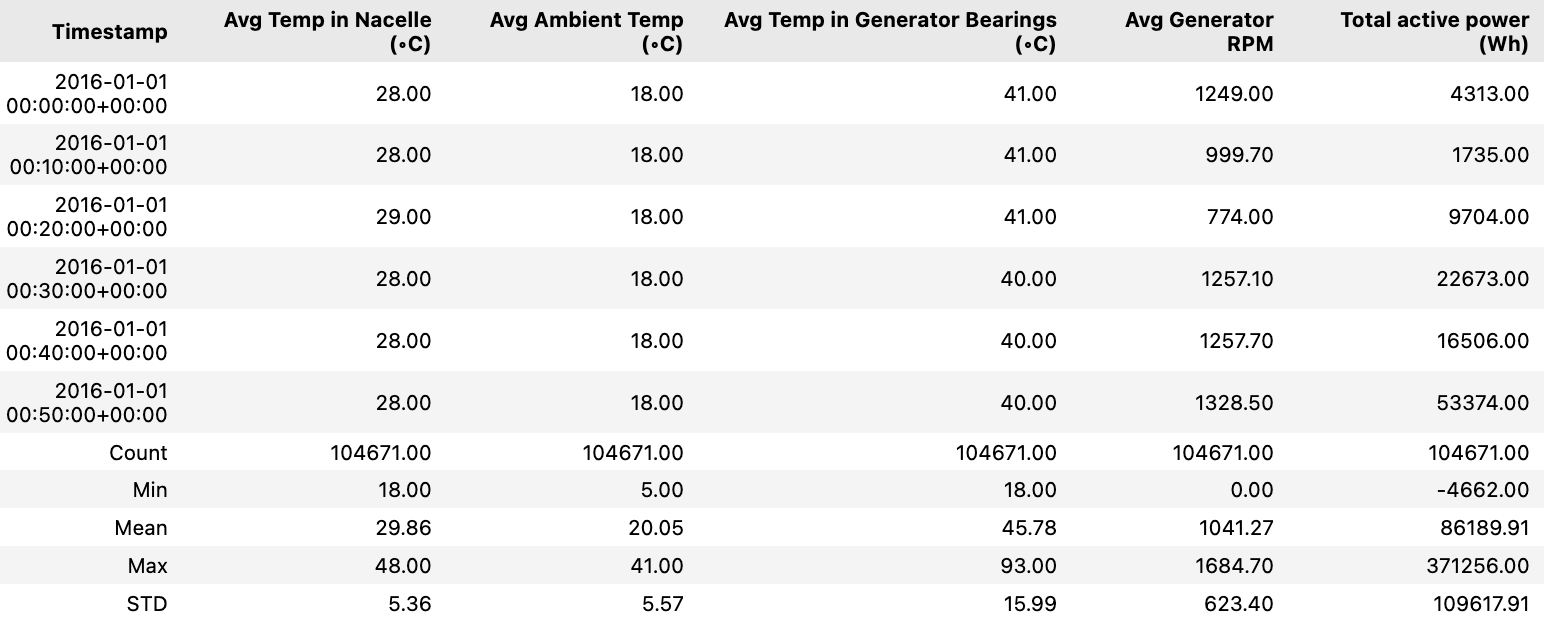
\includegraphics[scale=0.25]{Methods/Sample_Signals.png}
    \end{center}
    \caption{Sample dataset of selected signals from Turbine 01 and some statistics that describe the full dataset}
    \label{fig:sample_signals}
  \end{figure}

 \subsection{Logs}
  Some events are logged by the SCADA system in non-fixed intervals. The events recorded by the system are divided into three categories: Alarm log, 
  Warning log and Operation and System log. According to the VestasOnline Enterprise user manual \cite{voe}, alarms are system notifications that alert operators to 
  an error scenario that has forced a wind turbine to cease normal operation and transition to one of three operational states: Pause, Stop, or 
  Emergency (one of the following three acknowledgments is needed to resume operation: Local acknowledgment 
  from the controller unit of the turbine, Remote acknowledgment from VestasOnline®, or Automatic acknowledgment), 
  whereas warnings are system messages that indicate an irregularity that requires attention but does not cause the turbine 
  to immediately cease normal operation and exit the Run state.\\
  Operational logs are used to track a system's normal operation and to keep track of events and activities that have occurred. 
  These logs can be used by operators for troubleshooting purposes.\\
  System logs are used to monitor the operation and health of the system's hardware and software components. 
  These logs can be used to identify system problems, such as hardware failures or software faults, and can aid in diagnosing and resolving these problems.
  Table \ref{tab:logs} shows samples of logs from each category found in the EDP dataset.


  \begin{table}[H]
          \centering
      \begin{tabular}{|c|c|}
      \hline
          \textbf{Type of log event} & \textbf{Sample log event}  \\
          \hline
          \multirow{2}{12em}{\centering Alarm log} & \emph{"High temperature brake disc"} \\
          & \emph{"High pres offlin:\_\_\_\_RPM/ \_\_\_\degree C"} \\
          \hline
          \multirow{2}{12em}{\centering Warning log} & \emph{"Yaw Position is changed: \_\_\degree"} \\
          & \emph{"Low Battery Nacelle"} \\
          \hline
          \multirow{3}{12em}{\centering Operation and System log} & \emph{"External power ref.:\_\_\_\_kW"} \\
          & \emph{"GearoilCooler \_, gear: \_\_\_\degree C"} \\
          & \emph{"Pause pressed on keyboard"} \\
      \hline
      \end{tabular}
      \caption{Sample log events found in the EDP Logs dataset}
          \label{tab:metrics}
  \end{table}
  According to our analysis, we found around 180 different templates of log events in the ERP Logs dataset. A template, as demonstrated in Table \ref{tab:logs}, 
  describes a certain event and may or may not be parameterized. E.g., \emph{"External power ref.:2000kW"} and \emph{"External power ref.:1392kW"} report a similar event 
  (\emph{"External power ref.:\_\_\_\_kW"}) but with different parameters (kW production) and, hence, will be considered only once when calculating the total number of unique 
  templates found.

  \par As information is only logged when an event occurs, this dataset does not have a fixed frequency and it's hence difficult to statistically describe all the different 
  log templates found. Since our experiments were focused on generator bearings-related failures, we will describe further some of the log events found from the different
  categories that are related to the generator component. Those events were utilized in one of our proposed methods (see \ref{sub:dk_method}).
  In the Operation and System log of Turbine 09, the events \emph{"Gen. int. vent. \_, temp:\_\_\_\degree C"} (Event class I) and \emph{"Gen. ext. vent. \_, temp:\_\_\_\degree C"} (Event class II)
  occurred 1735 and 2026 times, respectively, with the following frequencies:
  \begin{table}[H]
    \centering
    \begin{tabular}{cc|c|}
      \cline{2-3}
      \multicolumn{1}{c|}{} & \textbf{Event class I} & \textbf{Event class II} \\
      \hline
      \multicolumn{1}{|c|}{Min frequency} & 1 second & 1 second \\
      \hline
      \multicolumn{1}{|c|}{Mean frequency} & 10 hours and 6.47 minutes & 8 hours and 39.48 minutes \\
      \hline
      \multicolumn{1}{|c|}{Max frequency} & 9 days and 40.82 minutes & 9 days and 41 minutes \\
      \hline
    \end{tabular}
    \caption{Measured frequencies of selected classes of log messages found in the Operation and System log of Turbine 09}
    \label{tab:OpSysLogsT09}
  \end{table}

  \begin{flushleft}
  Figure \ref{fig:sample_logs} shows a sample of those events.
  \end{flushleft}

  \begin{figure}[H]
    \begin{center}
      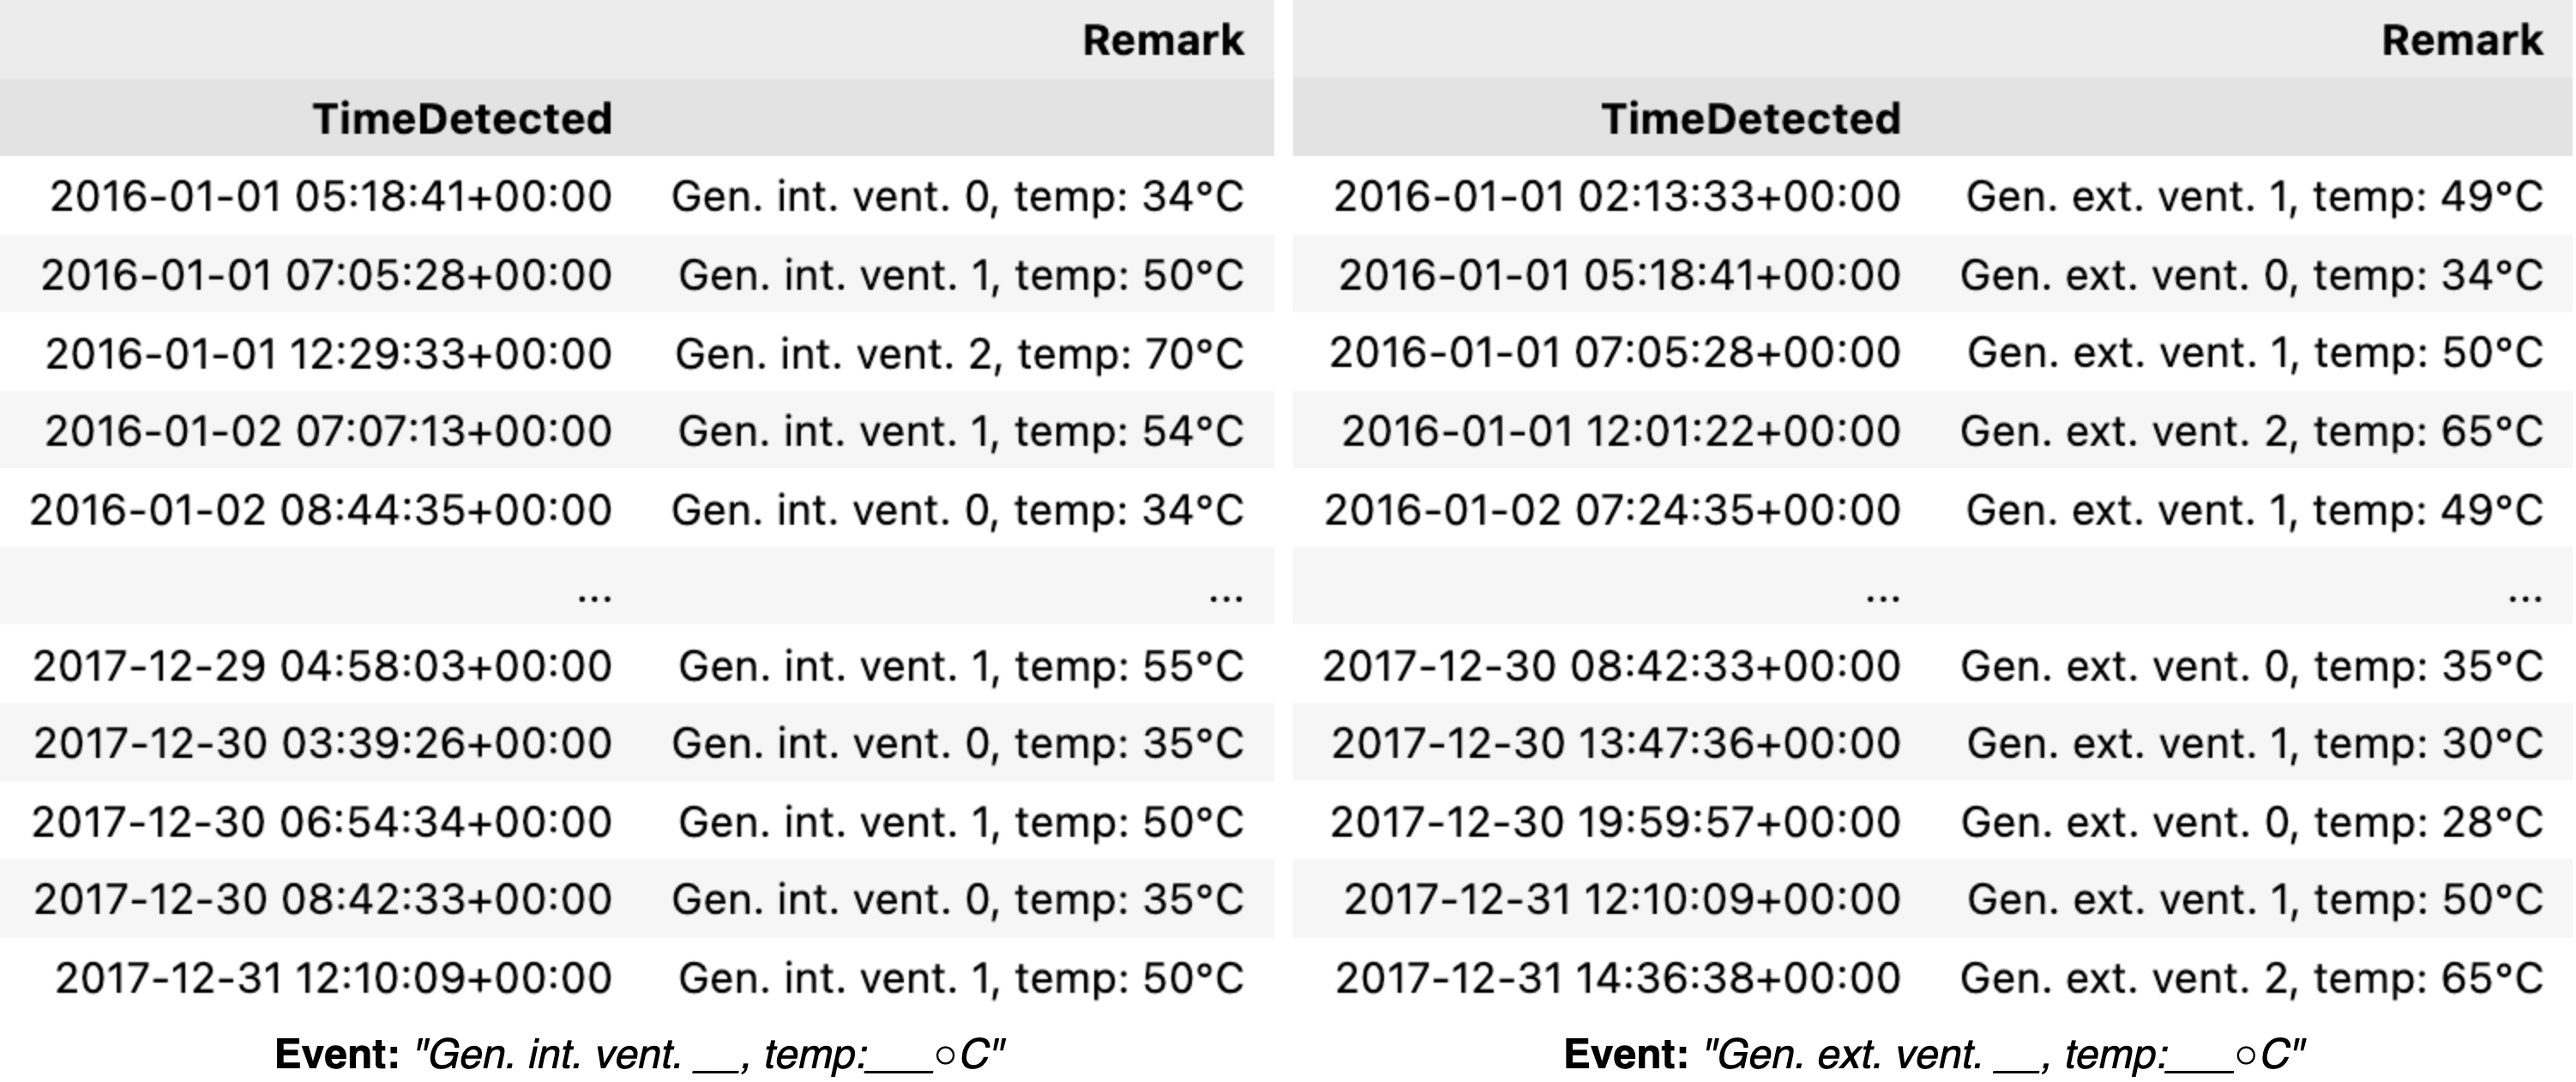
\includegraphics[scale=0.131]{Methods/Log_sample.png}
    \end{center}
    \caption{Sample messages found in the Operation and System Log of Turbine T09 from event class I and II, respectively}
    \label{fig:sample_logs}
  \end{figure}

  In the Alarm and Warning log of Turbine 09, the events \emph{"Hot generator \_\_\_\degree C \_\_\_\_\_\_kW"} (Event class III) and 
  \emph{"High temp. Gen bearing \_:\_\_\_ \degree C"} (Event class IV) occurred 899 and 31 times, respectively, with the following frequencies:
  \begin{table}[H]
    \centering
    \begin{tabular}{cc|c|}
      \cline{2-3}
      \multicolumn{1}{c|}{} & \textbf{Event class III} & \textbf{Event class IV} \\
      \hline
      \multicolumn{1}{|c|}{Min frequency} & 2 seconds & 1 hour and 13 minutes \\
      \hline
      \multicolumn{1}{|c|}{Mean frequency} & 10 hours and 27.31 minutes & 91 hours and 16.2 minutes \\
      \hline
      \multicolumn{1}{|c|}{Max frequency} & $\approx$ 281 days & $\approx$ 25 days \\
      \hline
    \end{tabular}
    \caption{Measured frequencies of selected classes of log messages found in the Alarm and Warning log of Turbine 09}
    \label{tab:AlrmWarnLogsT09}
  \end{table}

  \begin{flushleft}
  Figure \ref{fig:sample_warnings} shows a sample of those events.
  \end{flushleft}

  \begin{figure}[H]
    \begin{center}
      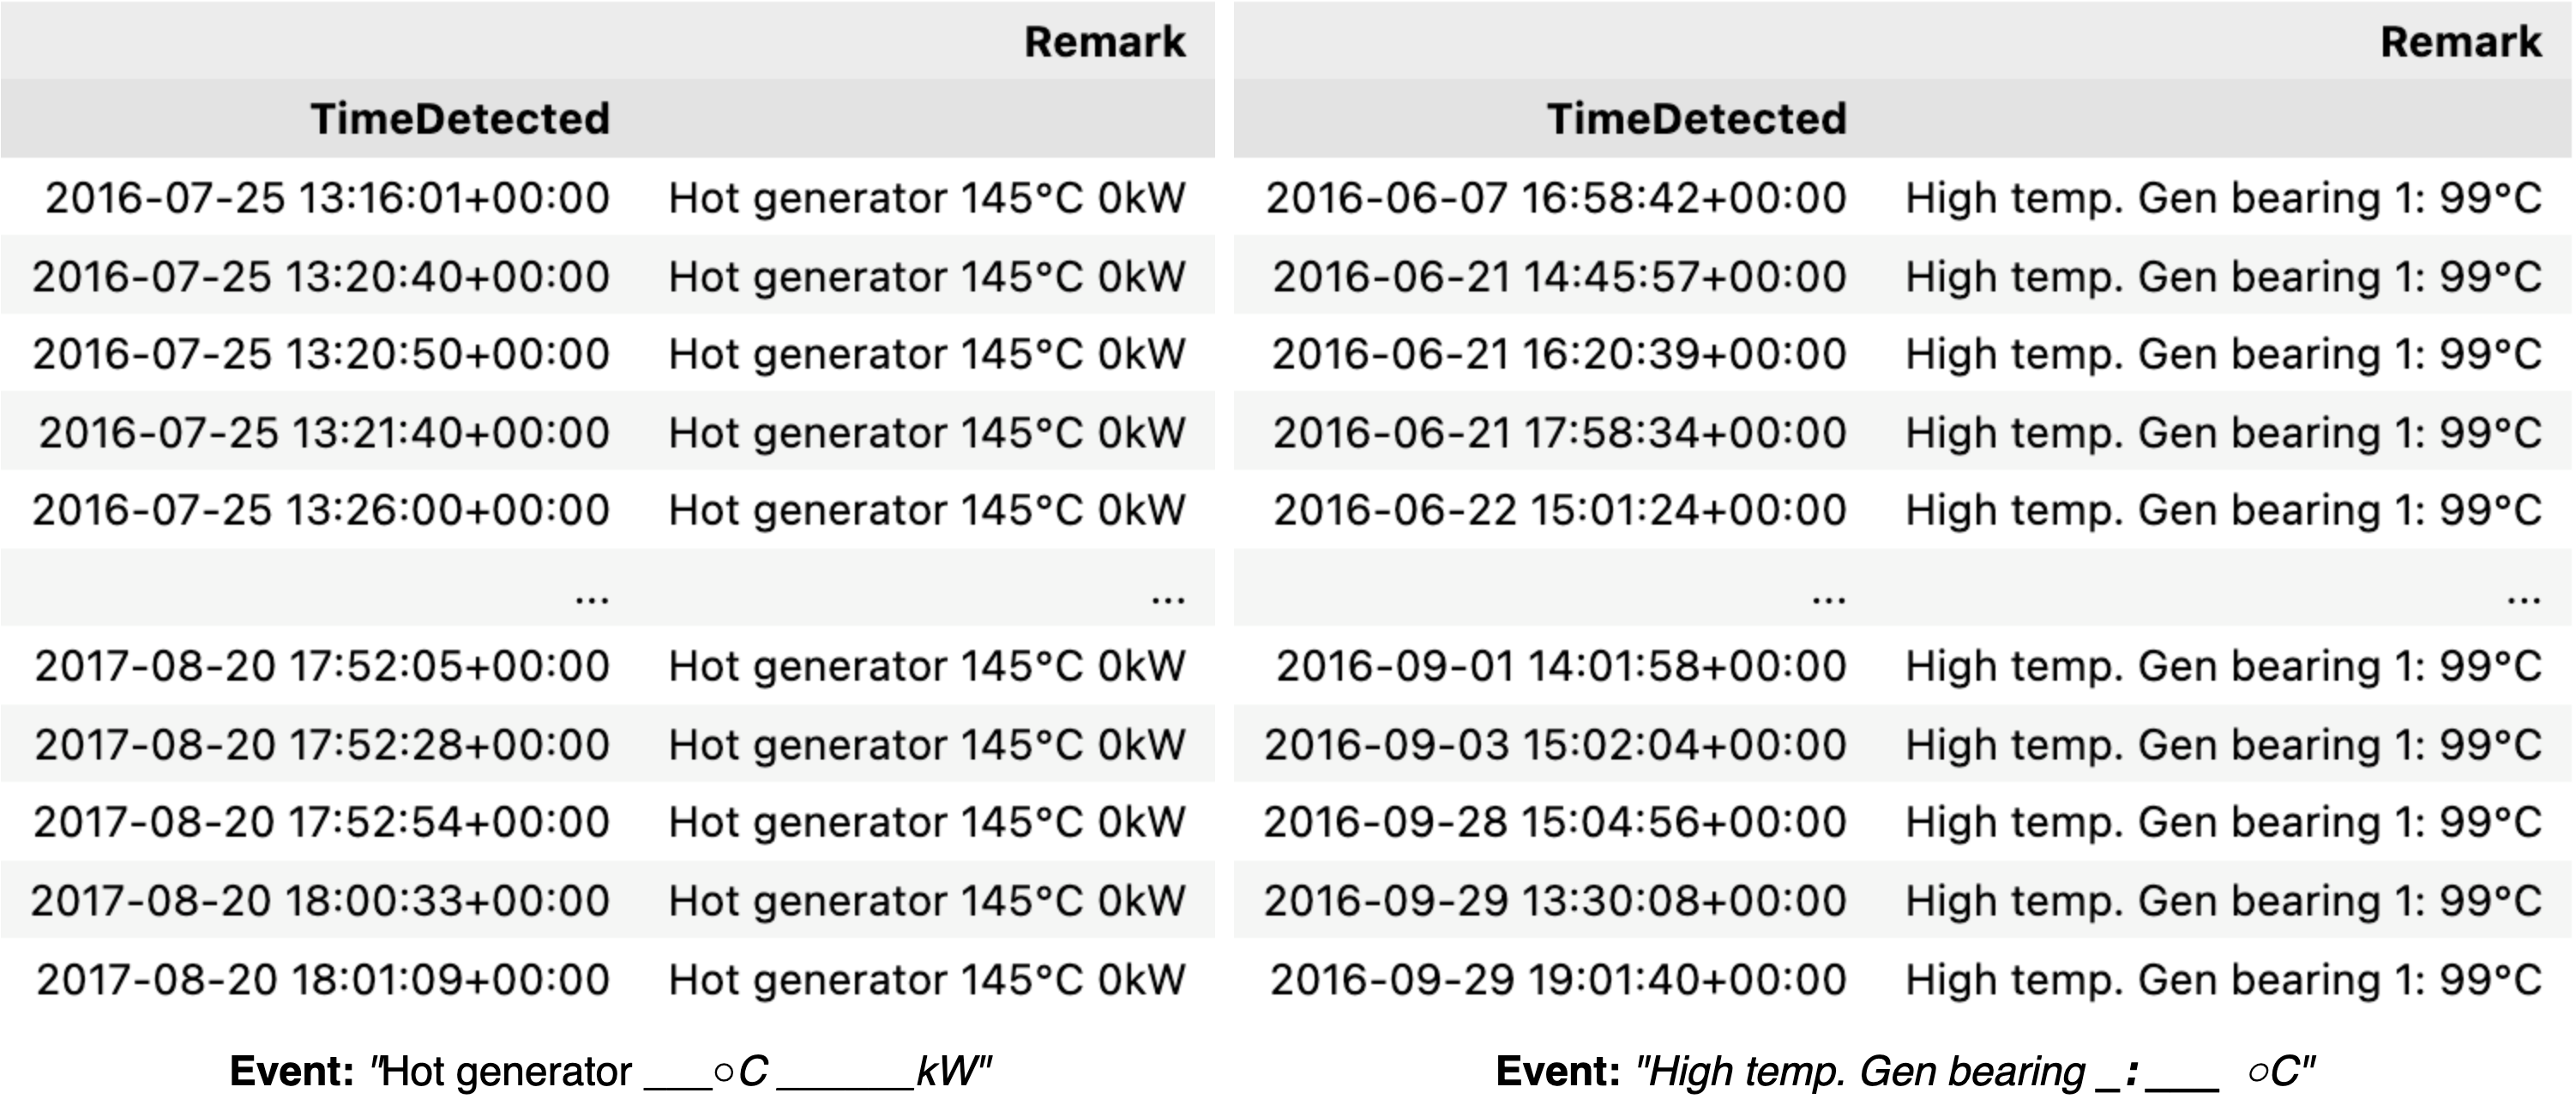
\includegraphics[scale=0.131]{Methods/Warning_sample.png}
    \end{center}
    \caption{Sample messages found in the Alarm and Warning Log of Turbine T09 from event class III and IV, respectively}
    \label{fig:sample_warnings}
  \end{figure}



\subsection{Failures}
  The Failures dataset contains the history of failures, inspections, or maintenance that occurred in the turbines and was manually recorded by technicians. 
  Each record reports the time of the event, component (e.g., Generator, Hydraulic group,..), and a text description of the failure 
  or event (e.g., "Generator replaced", "Oil leakage in Hub",..).\\ 
  This dataset was used in backtesting to validate the models' capability of detecting failures early. Table \ref{tab:failures} lists all the recorded failures found 
  in the EDP dataset.

\clearpage

\section{Normal behavior modeling}
According to Tautz-Weinert and Watson \cite{SCADA_NBM_Review}, Normal Behavior Modeling (NBM) detects anomalies in normal operation by empirically modeling an 
observed parameter based on a training phase. Figure \ref{fig:NBM} depicts the concept of model-based monitoring.
During operation, an anomaly is detected by deducting the value of the modeled signal ($\hat{y}$(t)) from the measured one (y(t))  and 
comparing the residual (e(t)) with a predefined threshold. If the threshold is exceeded, this signal is labeled as an anomaly.
There are two primary approaches for NBM: Full Signal ReConstruction (FSRC), in which only signals other than the target are utilized to predict the target, 
and AutoRegressive with eXogenous Input Modeling (ARX), in which previous values of the target are also employed.\\
Having defined NBM on an abstract level, we demonstrate next the machine learning models we used to generate modeled signals (y(t)) from input signals (x(t)) and 
then explain the anomaly detection approach we used. Given that the structure of the available signals (e.g., the number of signals and their frequency) varies based 
on the turbine's model, manufacturer and sensors installed, we defined the dataset used in this work in the previous section.

\begin{figure}[H]
  \begin{center}
    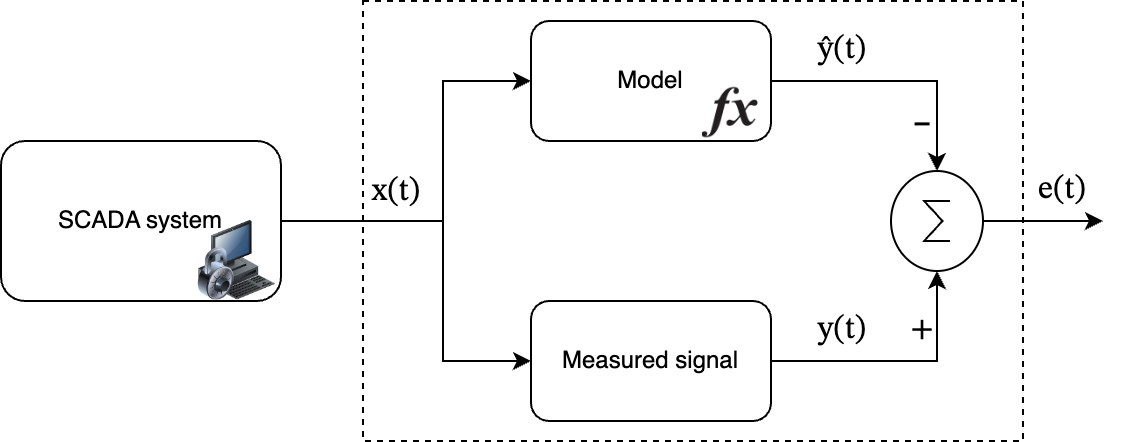
\includegraphics[scale=0.35]{Methods/NBM.png}
  \end{center}
  \caption{NBM with the input signals from the SCADA system (x(t)), measured signal (y(t)), modeled signal ($\hat{y}$(t)) and resulting error (e(t))}
  \label{fig:NBM}
\end{figure}

\subsection{Machine Learning in NBM}
  From a wide range of machine learning model types, NBM focuses on regression models \cite{Regression}. Regression models are part of the supervised learning family, 
  where the algorithm is trained on labeled data and the input features are mapped to corresponding output labels. 
  As opposed to classification models, where the algorithm predicts \emph{classes}, a regression model predicts numerical \emph{values} (dependent variables) from the input 
  features (independent variables).\\
  According to Tautz-Weinert and Watson \cite{SCADA_NBM_Review}, there are mainly three types of NBM regression models used in the research field: \emph{Linear and polynomial models},
  \emph{Artificial Neural Networks (ANNs)} and \emph{Fuzzy Systems}. Given their simplicity, we used linear models in the early phases of this work. Later on, we started using 
  ANNs for their capability of capturing non-linear dependencies in the data. We define these two types of models in detail in the next subsections.
  A fuzzy system \cite{Neuro_fuzzy} is an artificial intelligence system that employs fuzzy logic \cite{fuzzy_sets}. Fuzzy logic is a mathematical framework for 
  dealing with uncertainty and imprecision.
  The input and output variables in a fuzzy system are represented by fuzzy sets, which are collections of values with degrees of membership rather than tight boundaries. 
  The associations between the input variables and the output variables are then specified using fuzzy rules. 
  These rules are often represented as "if-then" statements, with the "if" section defining the input conditions and the "then" part defining the output actions.
  Training fuzzy systems was not within the scope of this work. However, we propose testing our methods on them in the future works section (see \ref{sec:future_works}).

  \subsubsection{Linear regression}
    Sir Francis Galton proposed the idea of linear regression in 1894 \cite{Natural_Inheritance}.
    Linear regression is used for analyzing the linear relationship between one or more independent variables and a dependent variable.
    The dependent variable must be continuous, whereas the independent variables can be continuous or categorical. For a dependent variable $Y$ and a set of $n$ independent
    variables $X_1$ through $X_n$, the linear regression equation is defined as follows:
    \begin{equation}
      Y = m_1X_1 + m_2X_2 + ... + m_nX_n + C
    \end{equation}
    where $m_1$ through $m_n$ and $C$ are constants. Figure \ref{fig:linear_regression} shows an example of linear regression for a single independent variable.

    \begin{figure}[H]
      \begin{center}
        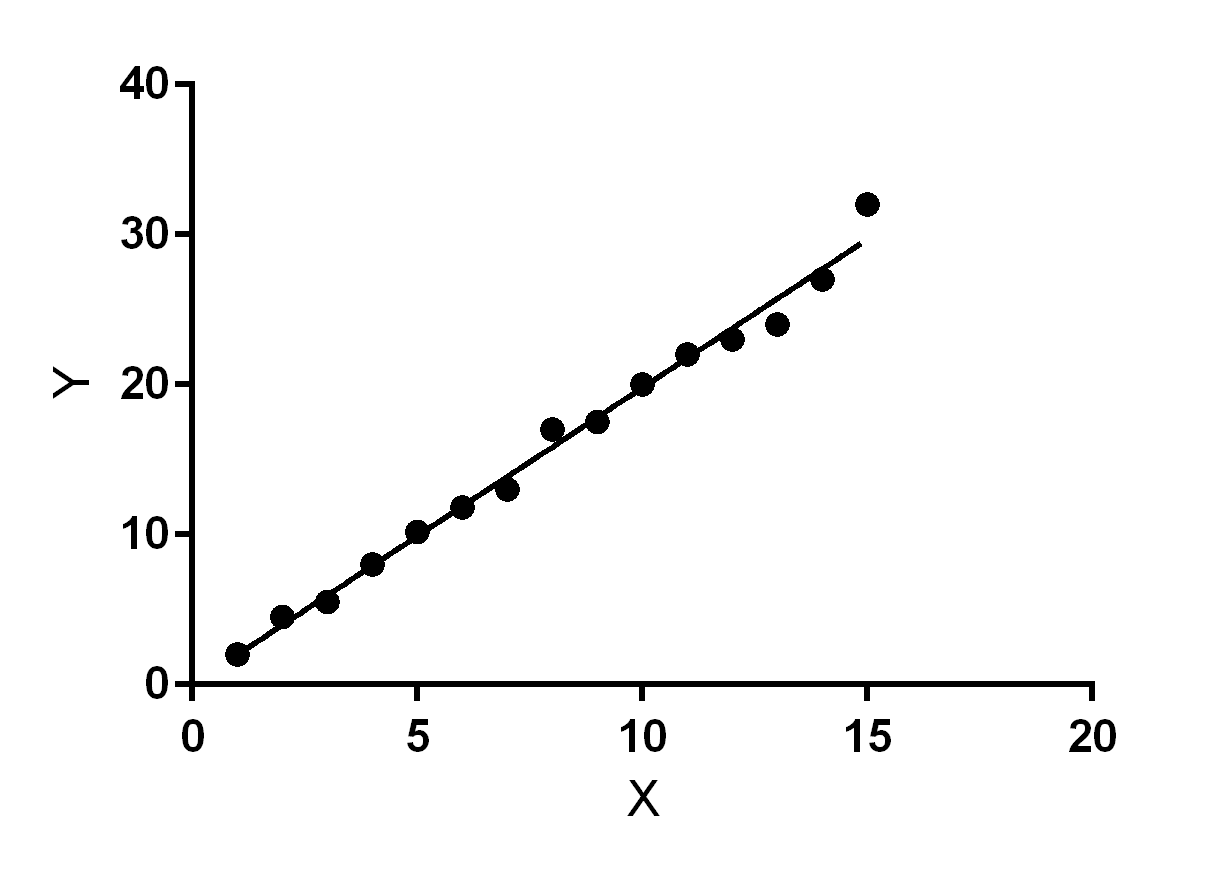
\includegraphics[scale=0.7]{Methods/Linear_regression.png}
      \end{center}
      \caption{Example linear regression with one dependent variable: $Y = mX + b$, where m and b are constants}
      \label{fig:linear_regression}
  \end{figure}

    When the relationship between the dependent variable and the independent variables is assumed to be linear, 
    linear regression is usually used. Linear regression is easy to use and understand, and it can be used to make predictions or find relationships between variables.\\
    In the example of normal behavior modeling for a wind turbine component, the dependent variable can be defined as the component's temperature 
    and the independent variables as a set of weather and turbine conditions measures (e.g., wind speed, ambient temperature, production value, other components' temperatures,..) 
    that have either a direct or indirect effect on the target component.
    NBM in its most basic form is based on linear or polynomial models \cite{SCADA_NBM_Review}. 
    Garlick et al. \cite{Garlick} employed a linear ARX model to detect generator bearings failures in bearing temperature measurements.
    Schlechtingen and Santos \cite{Schlechtingen} developed an FSRC linear condition monitoring model for the generator bearings' temperature.\\
    Although multiple linear regression models were also shown capable of fitting the data with high accuracy in many other applications (e.g., \cite{Linear_Regression_Example_1}), 
    they are, by definition, not capable of capturing more complex non-linear dependencies. In addition to that, linear regression may not be appropriate when there are a significant 
    number of independent variables. Artificial Neural Networks (ANNs) may be a better approach in these situations.


  \subsubsection{Artificial Neural Networks}
    Artificial Neural Networks (ANNs) are computational models that are inspired by the structure and function of biological neural networks in the brain \cite{NN_foundation}.
    They are made up of interconnected nodes (artificial neurons) that process and send data. 
    Pattern recognition, computer vision, natural language processing, and robotics have all made extensive use of ANNs 
    (for a comprehensive review of deep learning and neural networks, see \cite{Deep_learning_overview}, \cite{Goodfellow}).
    An artificial neuron, also known as a perceptron, is the fundamental building unit of a neural network. It is a mathematical function that accepts one or more input values 
    and outputs a single value \cite{Perceptron}.
    The input values are weighted, and the neuron applies an activation function to the total of the weighted inputs. The output value is subsequently passed on to the network's 
    other neurons. The activation function determines the neuron's output based on the input value(s) and weights.
    For a set of inputs $X_1$ through $X_n$, weights $w_1$ through $w_n$ and activation function $f$, the output of a perceptron $Y$ is calculcated as follows:
    \begin{equation}
      Y = f(\sum_{i=1}^n w_iX_i)
    \end{equation}
    The sigmoid function, the rectified linear unit (ReLU) function, and the hyperbolic tangent function are examples of common activation functions.
    Figure \ref{fig:Perceptron} shows a diagram of a perceptron.

    \begin{figure}[H]
      \begin{center}
        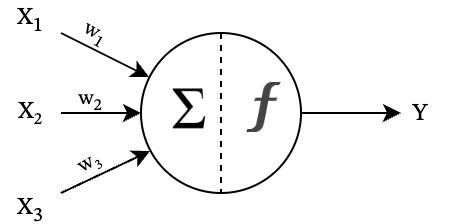
\includegraphics[scale=0.4]{Methods/Perceptron.png}
      \end{center}
      \caption{Example perceptron with three inputs}
      \label{fig:Perceptron}
    \end{figure}

    In the context of deep learning, an ANN consists of one input layer, one output layer and one or more \emph{hidden} layers.\\
    A hidden layer is a layer of neurons that is not connected directly to either the input or output layers. 
    It is referred to as "hidden" because its neurons are not visible to the outside world, implying that its calculations are not directly apparent from input or output.\\
    Information goes from the input layer, through one or more hidden layers, and then to the output layer in a \emph{feedforward} neural network, which is a type of ANN. 
    Each layer of neurons computes on the input data and sends the results to the next layer. The hidden layers extract and alter information from input data that can be 
    utilized to make predictions or choices.\\
    The number of hidden layers in an ANN is a hyperparameter that can be tuned during the training process.
    The number of hidden layers and neurons in each layer is determined by the task's complexity, the amount of accessible data, and the required level of accuracy.\\
    After obtaining better results with it compared to linear regression (see Experiment \ref{exp:I}), we decided to train the normal behavior models
    on a feed-forward neural network having the architecture shown in Fig. \ref{fig:MLP} using ReLU (firstly introduced by Fukushima \cite{Fukushima}) 
    as an activation function in the hidden layers and a linear activation function (input = output) in the output layer. 
    The output of the ReLU activation function is zero for any negative input, and for any positive input, the output is equal to the input.

    \begin{figure}[H]
      \begin{center}
        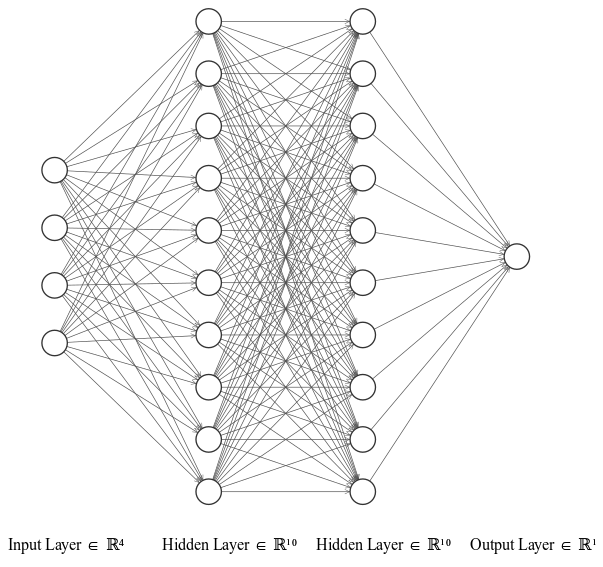
\includegraphics[scale=0.4]{Methods/MLP_cropped.png}
      \end{center}
      \caption{Architecture of normal behavior neural network model used in this work. \\
      \emph{The input layer shape will vary based on the experiment and the number of input features.}}
      \label{fig:MLP}
    \end{figure}

  \subsection{Reconstruction-based Anomaly detection}
    The main idea behind training and improving normal behavior models is to allow our models to detect anomalies more accurately.
    An anomaly is defined as an occurrence or observation that differs from what is expected, usual, or typical. 
    By comparing the observed data to a reference set, such as historical data or a pre-defined model, anomalies can be found.
    Positive and negative anomalies are also possible. In the context of wind
    turbine condition monitoring and when mainly monitoring temperatures of the system, we focus on positive anomalies because a component that is 
    overheating---due to wear and tear, oil leakage, faulty fan,\dots---is likely to fail. There is, however, no unified method in the research field to identify a data point 
    as an anomaly. Brandao et al. (\cite{Brandao_1}, \cite{Brandao_2}) used a fixed value of the mean absolute error as an anomaly threshold in their 
    gearbox and generator fault detection model, even though this number was particular and no longer valid following maintenance procedures. 
    Schlechtingen and Santos \cite{Schlechtingen} used daily average prediction errors in generator bearings temperature to trigger alarms. 
    Zhang and Wang \cite{Zhang_Wang} used a hard threshold of 1.5\degree C for the residual to identify anomalies in the main shaft rear bearing temperature.
    Bangalore and Tjernberg (\cite{Bangalore_1}, \cite{Bangalore_2}, \cite{Bangalore_3}) used a Mahalanobis distance to compare residual and target distributions from 
    the training period to find anomalies in gearbox bearings temperatures. The Mahalanobis distance was averaged over three days and compared to a training result-defined threshold.\\

    \par As there is no standard way to identify anomalies in temperatures in the context of condition monitoring for wind turbines using normal behavior models, we experimented 
    with several methods to do that and, finally, decided to set the anomaly threshold to the maximum prediction error seen in the training period. This way it is 
    guaranteed that the normal behavior models will not label any data point in the training dataset as an anomaly (complying with the assumption that the turbine was operating 
    in a healthy state during the training phase of the model) while having the threshold dynamically set based on the setup (e.g., 
    input and output features, training period, condition of the turbine during the training phase,\dots) without having to incorporate any domain knowledge related to the 
    specific component to-be-monitored. This also helped better compare different architectures of normal behavior models and the effect of incorporating the proposed log features, 
    not only in terms of prediction accuracy but also in terms of the quality and frequency of anomalies identified (a model that better fits the training data will have a 
    tighter anomaly threshold).

    \subsubsection{Anomaly vs Alarm}
    \label{subsub:anvsal}
      In our approach, we differentiate between \emph{Anomalies} and \emph{Alarms}. An anomaly is a data point that deviates from "normal", whereas an alarm is a proactive 
      way of communication that gets triggered when the operator's attention is urgently needed. The reason why we propose not to send an alarm every time an anomaly is 
      detected by the system is that we want our system to limit the number of false alarms as they are costly and counterproductive.\\
      As opposed to anomalies, which are tracked on a 10-min basis, we base alarms on daily events. If the number of anomalies found from the start of a day up until a given 
      point in time exceeds a certain threshold, an alarm is triggered. We set the \emph{alarm threshold} to the maximum number of 
      anomalies that occurred per day during the training period when using an \emph{anomaly threshold} set to the 99\textsuperscript{th} percentile of the distribution of the 
      training prediction errors. To summarize, an alarm can be defined as an anomaly in the number of system anomalies found per day.\\
  
  \subsection{Feature selection}
  \label{sub:featselect}
    The way the independent variables are chosen is usually done by measuring the correlation coefficients between available features in a
    dataset and the target feature and then selecting the features having a high correlation coefficient. Depending on the problem setting, other features can be also considered 
    based on domain knowledge, especially when dealing with a mechanical system as in the case of this work. A good example of this would be the incorporation of 
    the ambient temperature measurement as an input feature---even if it does not highly correlate with the target feature---to make sure that your model generalizes when 
    trying to predict a component's temperature throughout the year, by considering the effect of seasonality 
    (temperatures are expected to be higher in summer than in winter).\\
    In this work, we selected input features based on both domain knowledge and correlation coefficients. We used Kendall's method to measure the rank correlation \cite{Kendall}.
    In contrast to Pearson's correlation coefficient, Kendall's rank correlation can capture both linear and non-linear dependency between two variables by 
    measuring the monotonic relationship \cite{corr_comp}. Kendall's correlation factor ($\tau$) is calculated as follows:
    \begin{equation}
      \tau = \frac{C-D}{C+D}
    \end{equation}
    where $C$ is the number of concordant pairs and $D$ is the number of discordant pairs. Concordant pairs are observations in which the rankings of both variables increase or 
    decrease in the same direction, whereas discordant pairings are observations in which the ranks of both variables increase or decrease in opposing ways.
    The value of $\tau$ can range from -1 to 1, with -1 indicating a perfect negative relationship, 0 indicating no relationship, and 1 indicating a perfect positive relationship.\\
    As a result of our analysis, alongside the generated log embeddings/features (discussed in Section \ref{sec:LA}), the following sensor signals were used as 
    input features to the generator bearings normal behavior and condition monitoring models: 
    \emph{Average generator Revolutions Per Minute (RPM)}, \emph{Average temperature in the nacelle (\degree C)}, \emph{Total active power (Wh)} and 
    \emph{Average ambient temperature (\degree C)}. For the power curve condition monitoring models (discussed in \ref{subsub:PC}), 
    the \emph{Average windspeed within average timebase (m/s)} and \emph{Average ambient temperature (\degree C)} were the only features used to predict the power production values of 
    the turbine.

\clearpage
  
\section{Log analysis}
\label{sec:LA}
In this section, we will describe the different approaches we propose to utilize SCADA log messages and incorporate them into normal behavior models.\\
Most machine-learning architectures can only work with vector-shaped numerical inputs. Given that there are limited resources in the research field on how to generate 
numerical vectors from wind turbine SCADA system logs (see chapter \ref{chap:soa}), we introduce two methods that were proven capable of not only generating embeddings for 
machine-learning normal behavior models but also improving their accuracy (see chapter \ref{chap:experiments}): a domain-knowledge-based method and 
utilizing an open-source framework for analyzing log data called LogPAI. We will discuss each method in detail.

\subsection{Domain-knowledge-based method}
\label{sub:dk_method}

  \subsubsection{Creating log embeddings}
    We scanned through the different log messages available in the dataset looking for information that reflects the turbine state and might help the normal behavior model 
    fit the data more accurately. Since many normal behavior models monitor mechanical parts' temperature to mimic their thermal behavior, we narrowed the search down to operation and system logs
    that reflect events causing a change of temperature in major components. We, then, ended up with a category of logs that shows the states of internal or external ventilators
    of some components (see table \ref{tab:logs}). Being parts of the cooling systems of major components, fans or ventilators affect the components' temperature significantly.
    Therefore, log messages related to these are promising candidates.
    \begin{table}[H]
      \centering
      \begin{tabular}{|c|c|}
      \hline
       \textbf{Log text template} & \textbf{Log text sample}\\
       \hline
       Gen. ext. vent. \_, temp:\_\_\_\degree C & Gen. ext. vent. 2, temp:65\degree C \\
       Gen. int. vent. \_, temp:\_\_\_\degree C & Gen. int. vent. 1, temp:50\degree C \\
       HV Trafo. vent. \_, temp:\_\_\_\degree C & HV Trafo. vent. 0, temp:2\degree C \\
       Nac.vent.\_, nac/gear:\_\_\_/\_\_\_\degree C & Nac.vent.3, nac/gear:43/ 54\degree C \\
      \hline
    \end{tabular}
    \caption{Example log text templates with sample texts}
      \label{tab:logs}
    \end{table}

    Indeed, our analysis showed a clear relationship between the state of a ventilator and the temperature of its turbine component.
    As shown in Fig. \ref{fig:vent}, at low temperatures of the generator bearings, the internal ventilator will switch off. The bearings will then heat up which, in turn, causes
    the ventilator to turn on which cools the bearings down, and so on.

    \begin{figure}[H]
      \begin{center}
        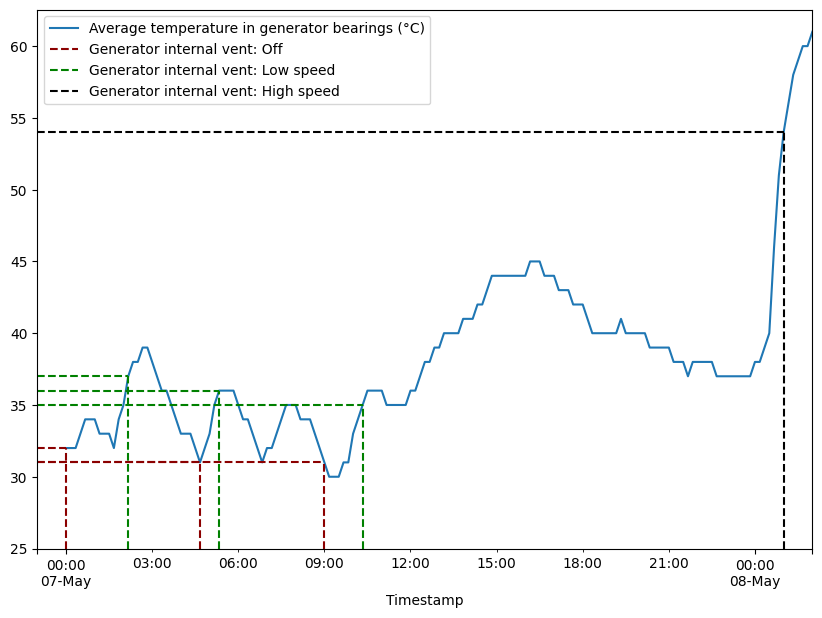
\includegraphics[scale=0.65]{Methods/Vent_Signals.png}
      \end{center}
      \caption{Generator internal vent control signals and their effect on the generator bearings temperature}
      \label{fig:vent}
    \end{figure}

    Analyzing the log texts of interest (e.g., \emph{Gen. ext. vent. 2, temp:65\degree C}), we deduce that they provide three pieces of information: 
    1. Description of the ventilator (e.g., \emph{Gen. ext. vent.}), 2. State of the ventilator (\emph{0, 1, 2 or 3}), 
    3. Temperature of the turbine component the ventilator is installed in (e.g., \emph{65\degree C}).
    Since the component temperature is regularly provided as a SCADA sensor signal, we decided to focus on the other two parts of the log messages. 
    Our proposed method simply filters log messages containing the word "vent." and creates a new feature for every ventilator found in the data having its state as a value.\\
    In contrast to the signals data fixed rate of occurrence (10 min), the generated log embeddings have an inconsistent frequency (the SCADA system creates a new log entry only 
    when a ventilator changes states). We join both datasets by taking the value of the last occurrence in the log embeddings vector within a 10-minute window relative to a signal reading.
    Gaps in the log feature columns in the resulting dataset are then filled by propagating the last valid observation forward to the next valid (a ventilator has the same state as long as it hasn't changed).
    Figure \ref{fig:log-merge} demonstrates an example of the join operation described. Gaps occurring on the first records of the resulting dataset are, however, not filled by this 
    method. These are then filled in the next step by taking an inverse value of the first-occurring non-empty value. This inverse value simply represents an estimation of 
    the previous state of a ventilator: e.g., 0 or 2 if the first recorded value was equal to 1. There are cases where the state of 
    a ventilator changes more than once in a 10-minute window. We handle those by calculating \emph{time-based weighted averages} in windows of 10 minutes and replace 
    the values---representing the ventilator states---of those individual timeframes by the weighted averages. The Time-based Weighted Average (TWA) is calculated as follows:
    \begin{equation}
      TWA = \sum_{i}^{n} v_i * w_i
    \end{equation}
    where $n$ is equal to the number of occurrences in a (10-min) time window, $v_i$ value (ventilator state) at the i\textsuperscript{th} occurrence, 
    and $w_i$ is the weight assigned to the i\textsuperscript{th} occurrence and is calculated, for a fixed time window (in seconds) $TW$ and 
    the number of seconds since the start of the time window at the i\textsuperscript{th} occurrence $S_i$, as follows:

    \begin{equation}
      w_i = \begin{cases}
        \frac{S_i}{TW}\ \ \ \ \ \ \ \ \text{if}\ n = 0\\
        \frac{S_i - S_{i-1}}{TW}\ \ \ \ \text{otherwise}
      \end{cases}
    \end{equation}


    Measuring the Kendall correlation factor between the generated log embeddings and all the signals of the turbines, we found that for every temperature signal, there is at least 
    one log embeddings feature that, on average, highly correlates ($Rank>0.5$) with it.

    \begin{figure}[H]
      \begin{center}
        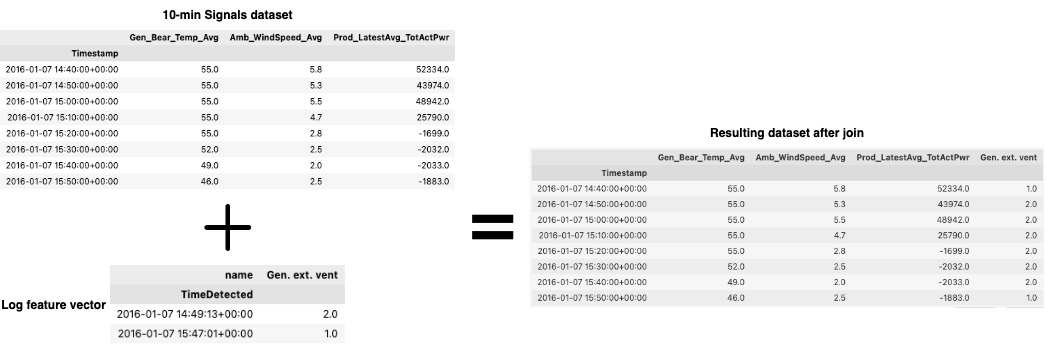
\includegraphics[scale=0.35]{Methods/Log_Merge.png}
      \end{center}
      \caption{Demonstration of the join operation between the signals 10-min dataset and a log embeddings vector}
      \label{fig:log-merge}
    \end{figure}

    \subsubsection{Data labeling and filtering}
    \label{subsub:PC}
      In this approach, we developed a method to improve SCADA-data-driven wind turbine power curve models 
      (for a comprehensive review of the various modeling techniques used to predict the power output of wind turbines and their applications in wind-based energy systems, 
      see \cite{Power_curves}). As shown in Figure \ref{fig:power_curve}.a, there are times when 
      the wind speed is above the turbine's cut-in speed\footnote{A turbine's cut-in speed is the wind speed at which the turbine's blades will start spinning, 
      as provided by the manufacturer in the turbine's datasheet} (4 m/s in this case), though the turbine's blades won't spin or will spin at lower rates than 
      normal. This could happen due to several reasons, including grid curtailment\footnote{Grid curtailment refers to the intentional reduction or restriction of power 
      generation from renewable energy sources due to limitations in the capacity of the electricity grid to accommodate the generated electricity.}, 
      the turbine being in a service state and/or manually stopped by the operator, or the turbine is simply underproducing due to technical failures.
      From a condition monitoring perspective, being informed that the turbine is underperforming when in an operating state is crucial as it's a sign 
      of a potential failure in one or more of the turbine's components. That is why, we introduce this method that focuses on isolating the data points collected 
      from the turbine's SCADA system when it's in operative mode. Handling the effect of grid curtailment on the turbine's performance is beyond
      the scope of this work, it's, however, discussed further in (TODO reference future works).\\
      
      We start by extracting the log messages that report the current state of operation; namely, logs containing one of the following regular expressions:
      \begin{bulletList}
        \item \emph{"Run"},
        \item \emph{"(Stop|Pause).*kW.*RPM"}, or
        \item \emph{"new SERVICE state"}
      \end{bulletList}
      The SCADA signals are then merged with the extracted log messages, using the same join strategy described in \ref{fig:log-merge}, and booleanly labeled based on the following logic:
      \begin{bulletList}
        \item Turbine's state of operation = \emph{"Run"}, if the log message contains the expression \emph{"Run"} or \emph{"new SERVICE state: 0"}
        \item Turbine's state of operation = \emph{"Stop"}, if the log message contains the expression \emph{"(Stop|Pause).*kW.*RPM"} or \emph{"new SERVICE state: 1"}
      \end{bulletList}

      Figure \ref{fig:power_curve}.b shows a sample power curve after labeling the data points based on the proposed method. 
      As shown, most of the time when the turbine isn't spinning, while the wind speed exceeds the cut-in speed, the data points are labeled 
      in red and would be filtered out. In addition to that, some periods when the turbine is in a transition phase from a running to a stopping state 
      will be filtered out. Those are also times when the turbine isn't necessarily underperforming but is gradually slowing down until it comes to a complete stop.
      One could argue that this proposed method could be simply replaced by filtering the data based on the turbine's rotor rotational speed 
      (if speed equals zero, then the turbine is not in operative mode). However, doing so wouldn't cover the transitional phases of the turbine, but simply 
      filter out the data at times when the turbine wasn't spinning regardless of the reason. This includes times when the turbine isn't spinning 
      due to a technical failure while in operation or due to low wind speeds.
      
      \begin{figure}[H]
        \begin{center}
          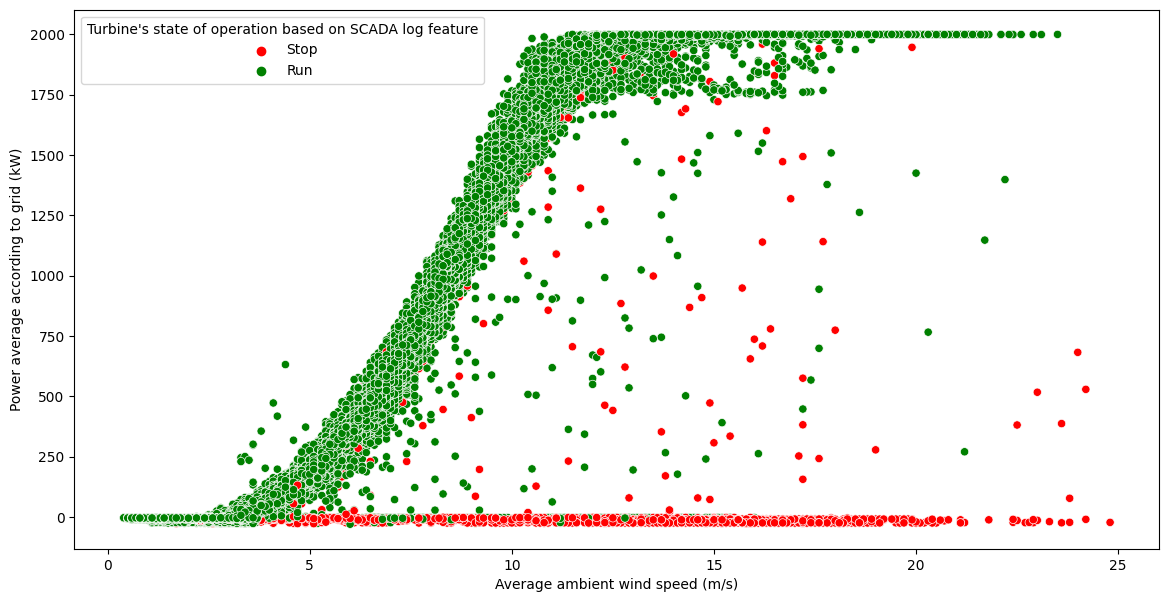
\includegraphics[scale=0.335]{Methods/power_curve.png}
        \end{center}
        \caption{Turbine 01 power curve with log-feature-based labels}
        \label{fig:power_curve}
      \end{figure}

      The log-based feature we introduced showed a clear improvement in the accuracy of power curve models (see experiment \ref{sec:Experiment IV}) when used to filter the data being input 
      to the normal behavior model (using data points having \emph{"Run"} as the state of operation exclusively). It also led to better results compared to 
      simply filtering by the rotor speed.
     

    \subsubsection{Visualization of warnings}
    \label{subsub:vis_warnings}
      Here, we introduced a straightforward yet effective way of visualizing (e.g., on an operation dashboard) messages from the Alarm and Warning logs that are relevant 
      to faults detected or predicted by normal behavior models and that are worth being reported to the operators.\\
      When the normal behavior model detects a fault in a certain turbine component, the SCADA logs are queried for messages reporting high temperatures in this component 
      during the same time window (e.g., last hour, last 12 hours, current day,\dots). If found, these messages could be included in the system reports that get sent to the operators
      to inform them of the detected failure. This gives more visibility and credibility to the detected/predicted failure by the system.\\
      Here, we use the following regular expression to filter relevant warnings and alarms in the SCADA log:
      \begin{equation}
        ((?=.*\text{Hot})(?=.*\{\}))|((?=.*\text{High temp})(?=.*\{\}))
      \end{equation}
      where the placeholder (\{\}) holds the abbreviation of the target major component as found in the signals dataset 
      (e.g., "Gen" for Generator and "Gear" for Gearbox). Figure \ref{fig:dashboard} shows an example of how these messages could be displayed 
      on a simple operation dashboard.

      \begin{figure}[H]
        \begin{center}
          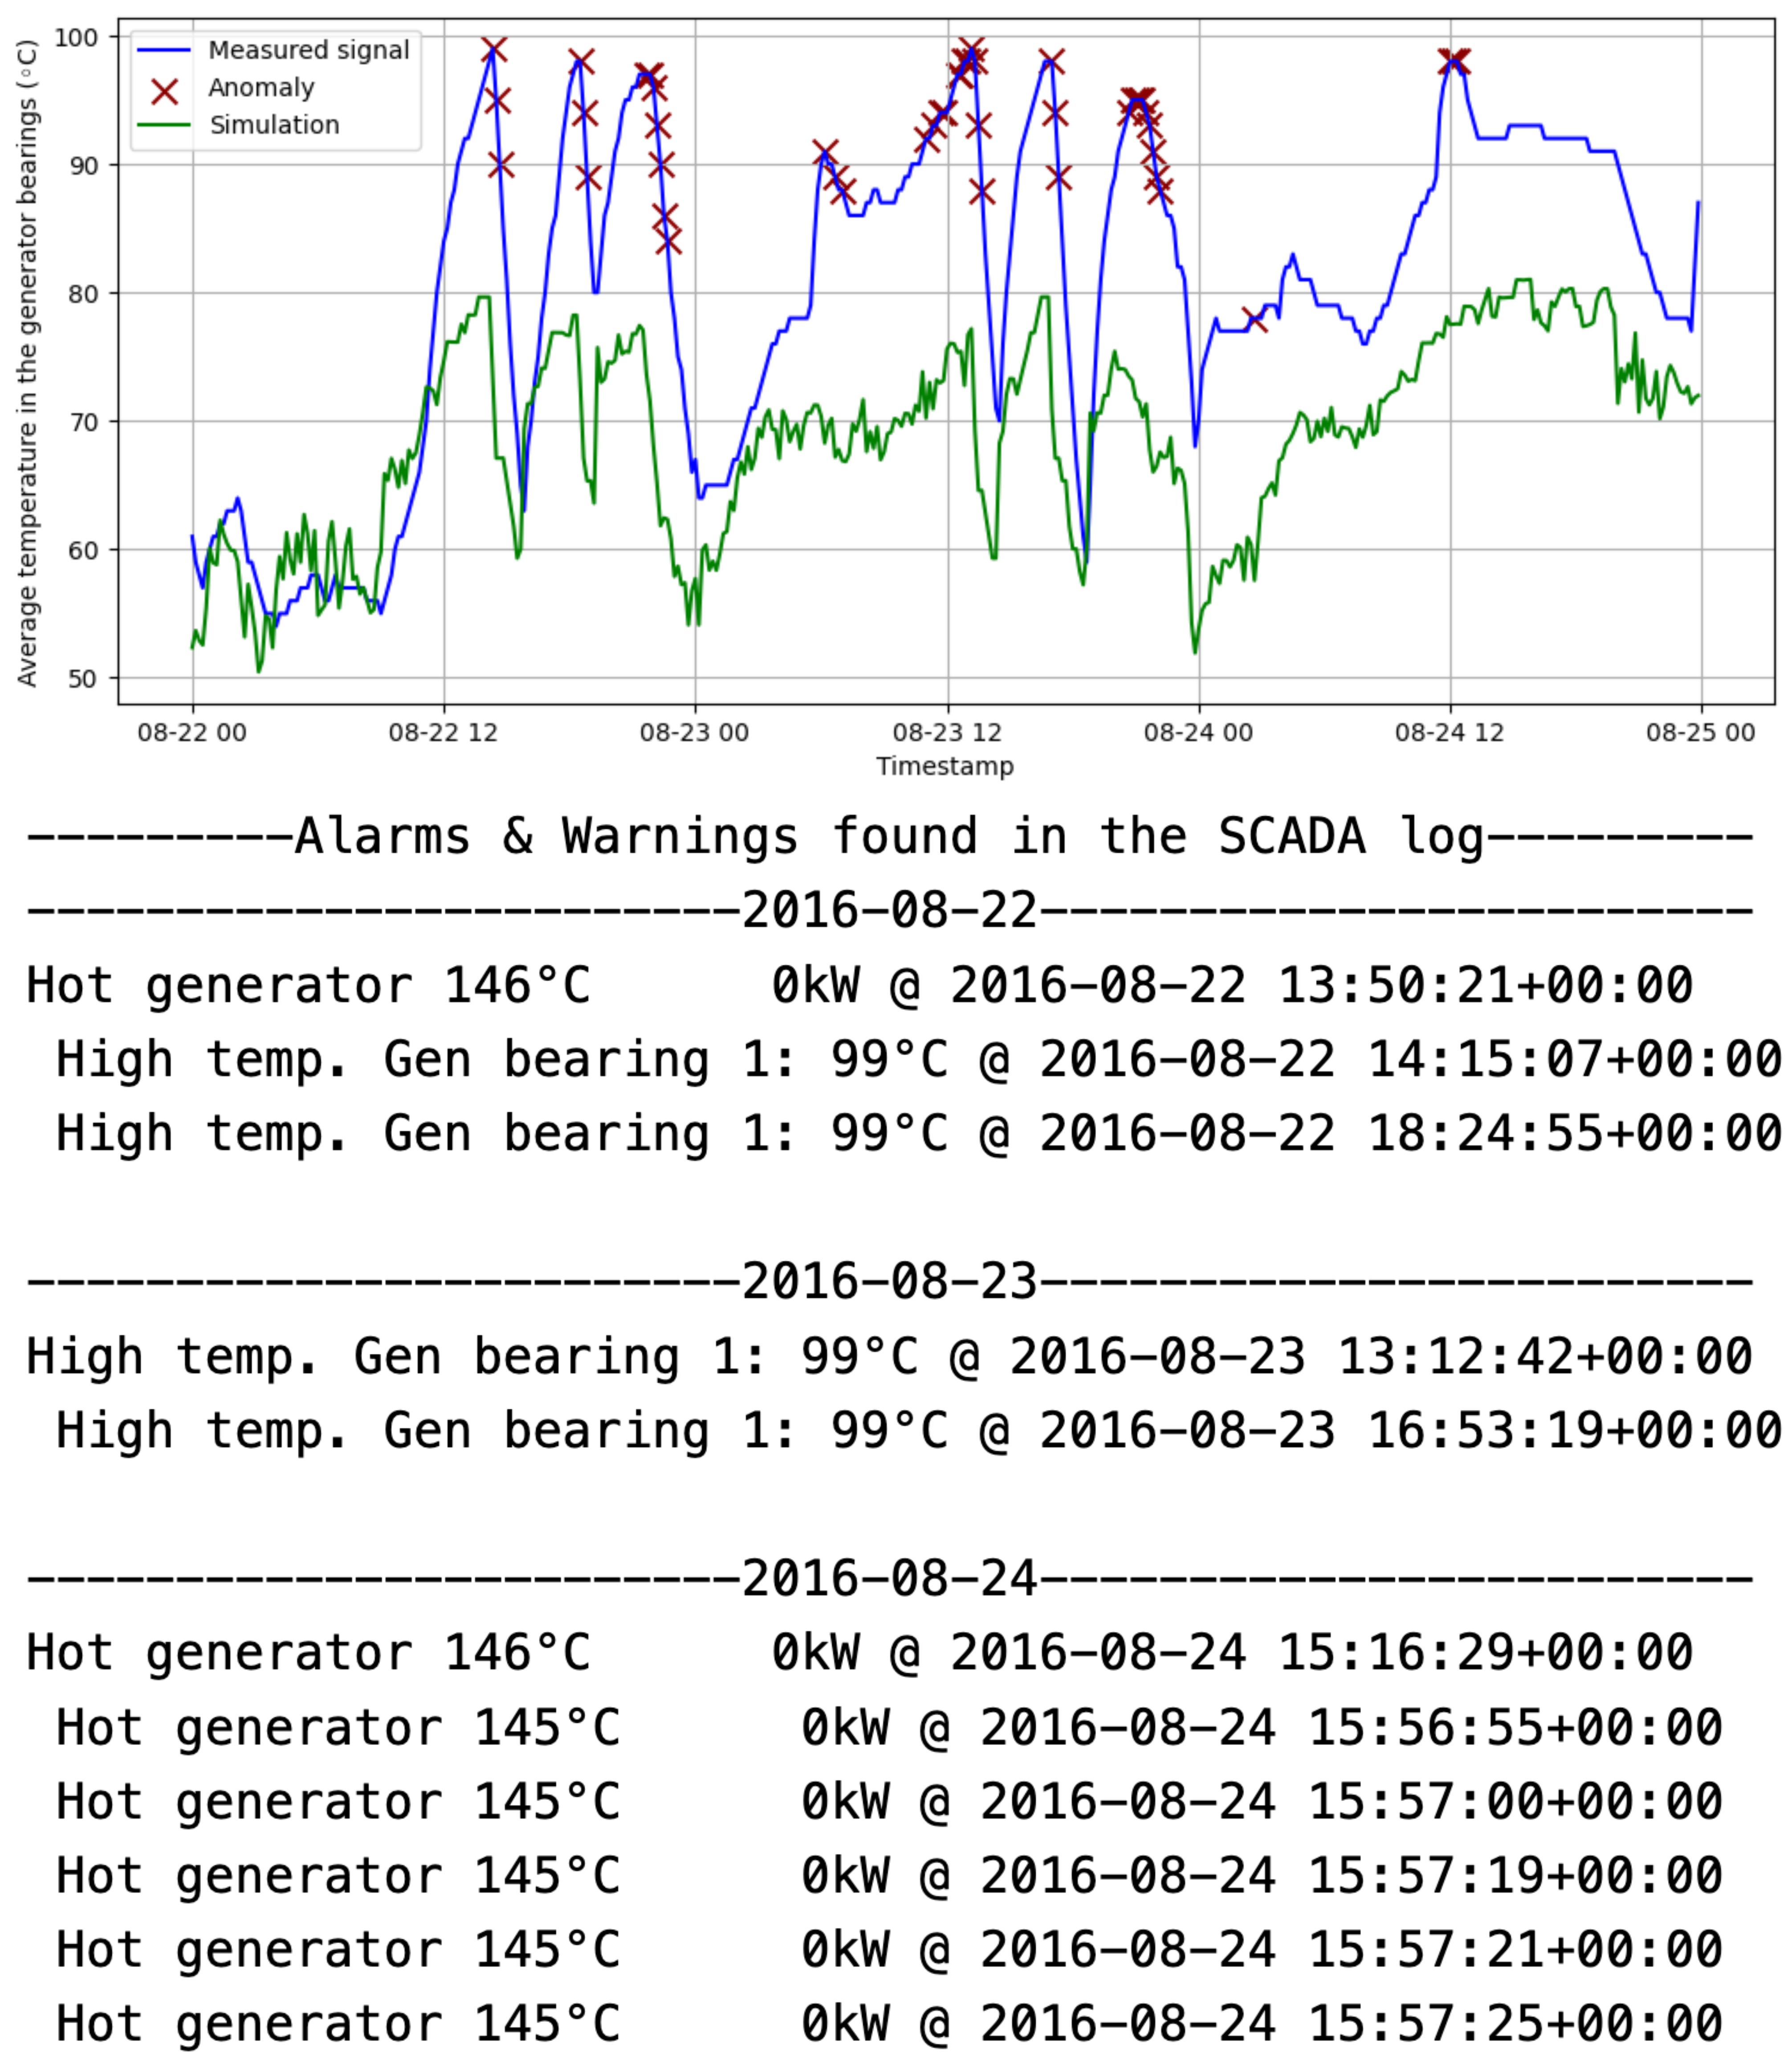
\includegraphics[scale=0.08]{Methods/Dashboard.png}
        \end{center}
        \caption{Example dashboard showing actual temperatures of the generator bearings (measured signal) against simulated signals 
        by a condition monitoring model (simulation). Anomalous data points are marked in red and relevant logs found are displayed at the bottom}
        \label{fig:dashboard}
      \end{figure}
    

  \subsection{Utilizing LogPAI}
    LogPAI (Log Analytics Powered by AI) is a study project and open-source platform for analyzing and managing log data \cite{LogPAI}. 
    Tsinghua University researchers started the project, which focuses on developing efficient algorithms and tools for log analysis, anomaly detection, and log data visualization.
    LogPAI includes a complete suite of log analysis and processing tools such as \emph{Logparser, Loglizer, and Logreduce}. 
    These applications can assist users in preprocessing and parsing raw log data, detecting anomalies and patterns, and summarizing log data concisely and understandably.
    We decided to utilize LogPAI's Logparser (\cite{Logparser_1}, \cite{Logparser_2}) and Loglizer \cite{Loglizer} to respectively parse and create numerical features from 
    SCADA logs in a more generic and automated way. While Logparser extracts structured information from unstructured log data generated by software systems automatically,
    Loglizer includes many feature extraction approaches for capturing the relevant information in log data and transforming it into a feature vector representation suitable 
    for machine learning-based log analysis. \\

      \subsubsection{Preprocessing of logs using Logparser}
        Logparser identifies and extracts relevant log events from raw logs (\cite{Logparser_1}, \cite{Logparser_2}). 
        It takes a log template-based method, grouping similar log messages to automatically learn and identify common structures and patterns in log messages. 
        It then creates log templates that represent the unique structure of the log data and utilizes them to parse and extract structured information from fresh log messages.
        Logparser is also adaptable, allowing users to create their log templates to meet their requirements.\\
        From the list of parsers available in the toolkit (e.g., LenMa \cite{LenMa}, LFA \cite{LFA}, LogSig \cite{LogSig},\dots), 
        we decided to use \emph{Drain} \cite{Drain} given that it is an online parser, which means it can process the SCADA logs 
        in real-time as they are generated. The Drain algorithm groups similar log messages together and extracts structured events from them using a 
        clustering-based approach by applying a two-stage approach: log parsing and event extraction.
        In the first stage, Drain employs a regular expression-based log parser to split raw log messages into a set of log keys and their related values. 
        The log keys are unique identifiers for each type of log message, whereas the log values are the specific information connected with each log message.
        It then uses a clustering-based approach in the second stage to group similar log messages together and extracts structured events from them. 
        Finally, Drain creates a template for each cluster that summarizes the relevant information contained in the log messages once the log messages have been clustered.
        The way this is done is by comparing the log keys and values of each log message using a similarity metric and assigning them to the best appropriate cluster based on 
        their similarity scores. The similarity metric $simSeq$ used by the algorithm is defined as follows:
        \begin{equation*} 
          simSeq=\frac{\sum_{i=1}^{n}equ(seq_{1}(i), seq_{2}(i))}{n}, \tag{1} 
        \end{equation*}
        where $seq_1$ represents a log message and $seq_2$ represents the log event of a log group/cluster. 
        $seq(i)$ is the i\textsuperscript{th} token of the sequence, $n$ is the log message length of the sequences and $equ$ is defined as follows:
        \begin{equation*} 
          equ(t_{1},\ t_{2})=
            \begin{cases} 
              1\ \ \ \ \text{if}\ t_{1}=t_{2} \\ 
              0\ \ \ \ \text{otherwise} 
            \end{cases} \tag{2} 
        \end{equation*}
        
        Applying Drain on the SCADA log data at hand by specifying its log format "\emph{<TimeDetected>,<TimeReset>,<UnitTitle>,<Content>,<UnitTitleDestination>}", we get 
        output structured log data (see Fig. \ref{fig:logparser} for an example) that the Loglizer can process to generate numerical features.

      \begin{figure}[H]
        \begin{center}
          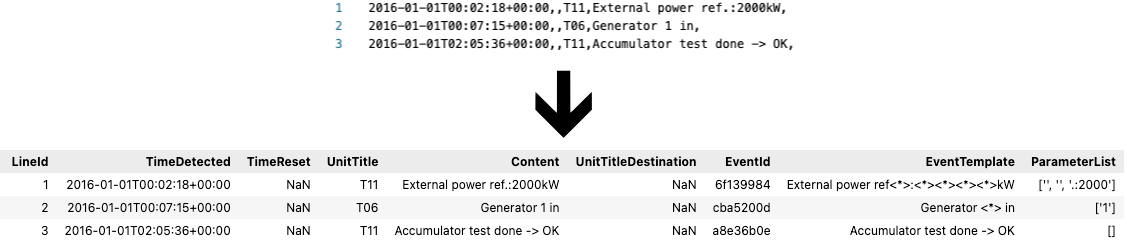
\includegraphics[scale=0.17]{Methods/Logparser.png}
        \end{center}
        \caption{Sample raw logs and their corresponding structured logs after being parsed by Logparser (Drain)}
        \label{fig:logparser}
      \end{figure}

        P.S. We filter out all log messages having the template \emph{} \emph{"External power ref.:\_\_\_kW"} before passing the logs to the Logparser
        as they weren't found to provide relevant information regarding the state of the turbine in the application of condition monitoring 
        of its generator (bearings). In addition to that, given their high volume and frequency, they were found to worsen the quality of 
        log embeddings generated by Loglizer when applied to our models.

      \subsubsection{Creating log embeddings using Loglizer}
        \label{subsub:Loglizer}
        Loglizer is a machine learning-based technique to log analysis created by Tsinghua University academics \cite{Loglizer}. 
        Several critical components comprise the technique, including feature extraction, feature selection, and anomaly detection.
        Loglizer collects numerous features from log messages in the first stage, such as token frequencies, Term Frequency-Inverse Document Frequency (TF-IDF) scores, 
        and structural features. 
        These features are then used to train a machine-learning model to learn the normal behavior of the system.
        In the second stage, Loglizer uses a feature selection algorithm to identify the most essential features.
        In the final step, Loglizer uses a machine learning algorithm to detect anomalous log messages. 
        The algorithm is trained on a labeled dataset that contains both normal and anomalous log messages. 
        During testing, the algorithm uses the learned model to predict whether each new log message is normal or anomalous based on the extracted features.\\
        Loglizer's \emph{Feature Extraction} component supports various feature extraction techniques, such as Bag-of-Words, TF-IDF, and Word2Vec, 
        to capture the essential information contained in log data. We utilized the Loglizer feature extractor, using TF-IDF \cite{TF-IDF} for term weighting, to generate numerical 
        features from the parsed logs.\\
        In natural language processing and information retrieval, TF-IDF is frequently used to assess how relevant a term is to a particular document within a collection 
        of documents \cite{tf-idf_review}. The TF component counts the number of times a phrase appears in a document and gives terms with more frequent occurrences a larger weight. 
        The IDF component calculates the rarity or frequency of each term across all documents in a collection and gives less frequent terms a larger weight.
        The equation for calculating the TF-IDF score of a term in a document can be expressed as follows:
        \begin{equation}
          TF-IDF(t,d,D) = TF(t,d) * IDF(t,D)
        \end{equation}
        where $t$ is a term in a document, $d$ a document in a collection of documents, $D$ the entire collection of documents, $TF(t,d)$ the term frequency of term $t$ in document $d$
        (the number of times term $t$ appears in document $d$) and $IDF(t,D)$ the inverse document frequency of term $t$ across all documents in collection $D$, defined as:
        \begin{equation}
          IDF(t,D) = log(\frac{N}{df(t)})
        \end{equation}
        , where $N$ is the total number of documents in $D$ and $df(t)$ is the number of documents in $D$ that contain the term $t$.\\
        We applied the feature extractor on the parsed \emph{Event IDs}---given that they uniquely describe the different events recorded in the SCADA log---and 
        used the generated features as input features to our normal behavior models. We also experimented with generating additional features by applying the Loglizer feature extractor 
        on the parsed \emph{Parameter lists}; those are used to parametrize the event templates which are, in turn, used to generate the Event IDs. 
        However, our models didn't show any improvements as a result of incorporating those additional features. Hence, we decided to stick to the Event ID-based 
        generated features only in our experiments.



\clearpage

\section{Summary}
TODO:
PUSH TO THE TOP\\
Diagram of all methods put together: ML model + log feature + Anomaly detection + Alarms,...

\clearpage